\documentclass[11pt,a4paper]{article}

\usepackage[spanish]{babel}
\usepackage{amsmath,amsfonts, amssymb, amsthm} % Podemos añadir amssymb, amsthm o bm
\usepackage{graphicx, tikz, xparse, array}
\usepackage[top=2cm,bottom=2cm,left=3cm,right=3cm,marginparwidth=1.75cm]{geometry} % Este paquete permite modificar los márgenes del documento
\usepackage[colorlinks=true, allcolors=blue]{hyperref} % Se indica que los hipervínculos van todos en azul
\usepackage{setspace}
\usepackage{caption}
\usepackage{xcolor}
\usepackage{graphicx} % Paquete para incluir imágenes
\usepackage{fancyhdr} % Paquete para cabeceras y pies de página
\usepackage{lipsum}   % Para generar texto de ejemplo
\usepackage[most]{tcolorbox}

\tcbuselibrary{breakable}


%Colores
\definecolor{verdeSuave}{HTML}{6AD58A}
\definecolor{verdeFuerte}{HTML}{206936}
\definecolor{blanco}{HTML}{FFFFFF}
\definecolor{negro}{HTML}{000000}
\definecolor{azulSuave}{HTML}{6ac9d5}
\definecolor{naranjaSuave}{HTML}{d5c06a}
\definecolor{rojoSuave}{HTML}{EF4949}
\definecolor{amarilloSuave}{HTML}{D8E058}


\setstretch{1.2}
\decimalpoint


%\graphicspath{ {images/}}

\title{\textbf{Tema 1: } Teoría de curvas}
\author{Mateo Rama García}


%\date{Fecha}

\begin{document}
  
\begin{titlepage}
  \centering  
  \vspace*{1cm}  % Espacio opcional antes de la imagen
  
\includegraphics[width=0.3\textwidth]{uniovi.jpg} \hspace{2cm}
  
\includegraphics[width=0.3\textwidth]{descarga.jpeg} \\[1cm] 
  \vspace{\fill}% Imagen centrada arriba
  \hrule
  \vspace{0.5cm}
  {\Huge \bfseries Trabajo en grupo\par}
  \vspace{0.5cm}
  {\Large \bfseries Fase I\par}
  \vspace{0.5cm}
  \hrule
  \vspace{1cm}
  {\bfseries PL3-B \\ [3ex]
  Andrés Fernández-Junquera Fernández UO302806\\[3ex]
  Bruno Martín Rivera UO302144\\[3ex]
  Javier Ortín Rodenas UO299855\\[3ex]
  Mateo Rama García UO300710\par} % Nombres centrados
  \vspace{\fill}  % Espacio después de los nombres
  {\Large \textbf{Fundamentos de computadores y redes}\par}
\end{titlepage}



\newpage

\tableofcontents

\newpage


\section{Primera parte}
\subsection{PasswordControl()}
Antes de nada defino una constante maxChars con valor 20 para la longitud de los arrays de caracteres que usemos. Estas cadenas solo podrán contener hasta 19 caracteres útiles debido al espacio necesario para \(\backslash \texttt{0}\) que indica el final de la cadena.

Para la primera parte del método, declaro un array de caracteres input1 y almaceno en él la primera entrada del usuario. Luego, uso la función strcmp para comparar la entrada con la contraseña. En caso de que sea distinto de 0 es que son diferentes, y prohíbo la entrada.

Para la segunda parte, guardo la nueva entrada del usuario en el array de caracteres input2. Luego, compruebo si la longitud del array es menor que 15 o si no coinciden los caracteres en las posiciones 8 y 5. En caso de que no se cumplan alguno de estos, aviso de que se ha producido un fallo.

\begin{itemize}
  \item Entrada válida: \(\texttt{input1 = \text{''abcdeighijklmnop''}, \hspace{1.5mm} input2 = \text{''aaaaabaabaaaaaa''}}\)
  \item Entrada no válida: \(\texttt{input1 = \text{''abcd''}, \hspace{1.5mm} input2 = \text{''abcdefghijklmnop''}}\)
\end{itemize}
\subsection{CountActiveBits()}
Esta función debe pedir dos números enteros sin singo. Posteriormente, debe contar el número de bits activos
que hay en cada número entre la posición 5 y la 8, ambos inclusive. Finalmente, en caso de que el 
número de bits activos entre las posiciones 5 y 8 de los dos números   no sea igual, la función 
imprimirá 'No coinciden' y llamará a la función exit().
\begin{itemize}
  \item Entrada válida: \(a = 352 \text{ y } b = 448\)
  \item Entrada no válida: \(a = 352 \text{ y } b = 0\)
\end{itemize}
\subsection{AsmBasedControl()}
\hspace{1mm}
Esta función debe leer tres enteros y pasárselos a IsValidAssembly.
Según la parametrización original del enunciado, esta segunda función debe comprobar que se
cumplan las dos condiciones siguientes:
\begin{itemize}
    \item El bit 8 del segundo número es igual al bit 5 del tercer número
    \item El valor de los 2 bits más bajos del primer número interpretados como 
        binario natural es mayor que 11
\end{itemize}
Como la codificación de 11 en binario natural es 1011b, la segunda condición no puede
ocurrir nunca en estas condiciones. Por tanto, escribimos la función para que tome los 4 bits
más bajos del primer entero, los interprete como natural, y lo compare con 11.
\begin{itemize}
  \item  Entrada válida: \(a = -3, \hspace{1.5mm} b = 403, \hspace{1.5mm} c = 56\)
  \item Entrada no válida: \(a = 1, \hspace{1.5mm} b = 7, \hspace{1.5mm} c = 5\)
\end{itemize}

\subsection{ArrayMinMax()}
Este función crea un vector de 3 posiciones de elementos de 8 bits. Después, 
pide por consola los valores para asignar en el mismo, restringiendo los valores de entrada a 
números enteros entre -128 y 127, es decir, los valores enteros codificables con 8 bits con la codificación de complemento a 2. 
Si la entrada no es válida, se informará por consola y se pedirá de nuevo un valor. 
\vspace{2ex}

Tras esto, calcula y muestra por consola tanto el valor máximo como el mínimo de los elementos del vector introducidos.
 Si la diferencia entre estos valores no es inferior a 2*ID[2] (en nuestro caso 2*9=18), se mostrará por pantalla el mensaje ''Fallo'' y se llamará a exit. 
 \begin{itemize}
  \item Entrada válida: \(a = -2, \hspace{1.5mm} b = 7, \hspace{1.5mm} c = 6\)
  \item Entrada no válida: \(a = 2, \hspace{1.5mm} b = 5, \hspace{1.5mm} c = -20\)
\end{itemize}
\newpage
\section{Segunda parte}
\subsection{Dirección de memoria IsValidAssembly}
Para responder a la pregunta, ponemos un punto de interrupción junto antes de la llamada a la
función IsValidAssembly. A continuación, ejecutamos el programa y en Visual Studio 2022. Para poder saber las 
direcciones de memoria, debemos ir a \textbf{Depurar \(\rightarrow\) Ventanas \(\rightarrow\) Desensamblado}. En esta ventana, 
podemos ver las direcciones de memoria a partir de las cuales se sitúa el código de paso de parámetros a la función IsValidAssembly.

\vspace{1ex}
\indent Buscamos la línea de código en la que se realiza la llamada a la función IsValidAssembly. Debajo de la llamada a esta función,
nos encontramos con la primera dirección de memoria a partir de la cuál se sitúa el código de paso de parámetros a la 
función IsValidAssembly. En nuestro caso, la dirección de memoria es \(\mathbf{004011E7}\). Como se puede observar en la siguiente imagen.
\begin{center}
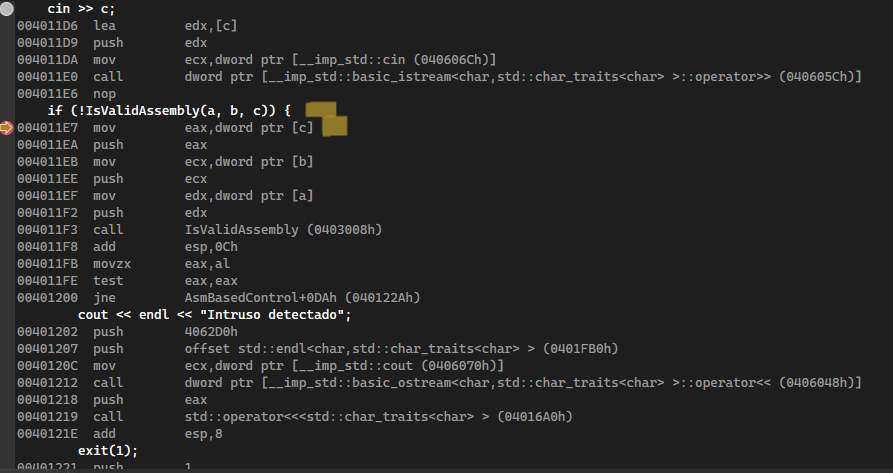
\includegraphics[width=\textwidth]{direccionIsValid.PNG}
\end{center}
\vspace{1ex}

\indent Para poder ver el código máquina y los mnemónicos de la función IsValidAssembly, debemos realizar la ejecución hasta llegar
al punto de interrupción que hemos puesto antes de la llamada a la función IsValidAssembly. Una vez llegamos a este punto, pulsamos la 
tecla F11 para ir al código en ensamblador, posteriormente pulsamos click derecho y pulsamos la opción \textbf{Mostrar bytes de código}. 
Así, podemos ver tanto los mnemónicos como las instrucciones en código máquina codificado en hexadecimal de la función IsValidAssembly. Como se muestra en las siguientes imagenes.
\begin{center}
  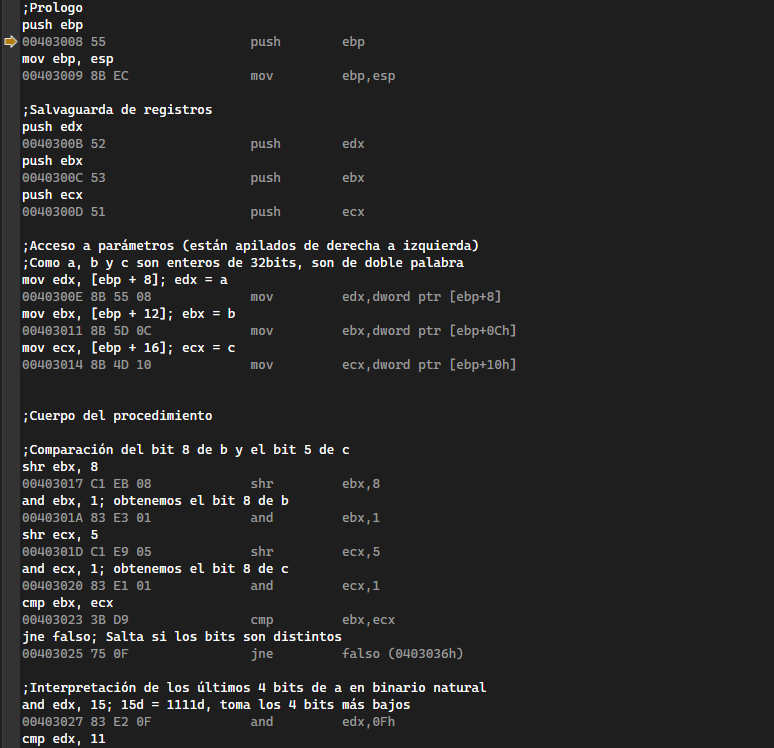
\includegraphics[width=0.8\textwidth]{codigomaquina2.png}
  \end{center}
\begin{center}
  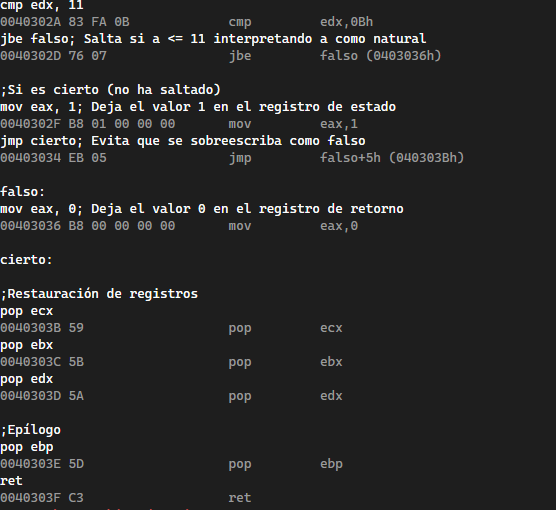
\includegraphics[width= 0.8\textwidth]{codigomaquina1 (1).png}
  \end{center}
\newpage
\subsection{Dirección de memoria PasswordControl}
En nuestro caso, la función de PasswordControl lee dos cadenas de la terminal, por la ambigüedad de la pregunta, 
ya que no sabemos con certeza a cual de las dos cadenas se refiere, hemos decidido mostrar ambas direcciones de memoria.

Para saber la dirección de memoria de la cadena que se lee en la primera función, debemos poner un punto de ejecución 
después de leer la cadena por terminal. A continuación, ejecutamos el programa en modo depuración y hacemos click 
en la opción \textbf{Ventanas \(\rightarrow\) Depurar \(\rightarrow\) Inspección}. Después de esto añadimos a Inspección 
la variable que contiene la cadena de caracteres y \(\& a\) para así, saber la dirección de memoria de la cadena. En nuestro caso, obtenemos lo siguiente:
\begin{center}
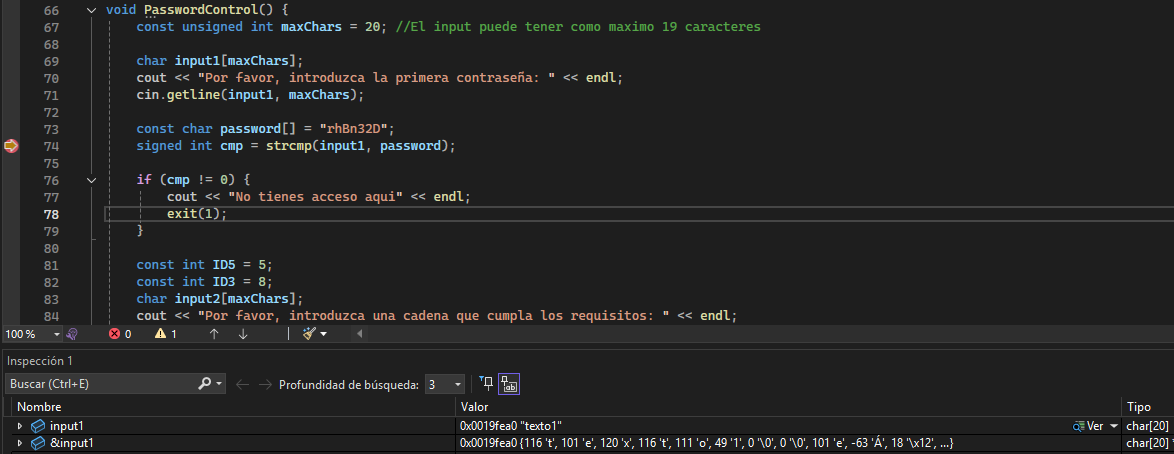
\includegraphics[width=\textwidth]{texto1.png}
\end{center}
Para verlo en memoria, debemos ir a \textbf{Depurar \(\rightarrow\) Ventanas \(\rightarrow\) Memoria}. En esta ventana,
introducimos \(\& a\), para así poder verlo almacenado en memoria. Como se muestra en la siguiente imagen.
\begin{center}
  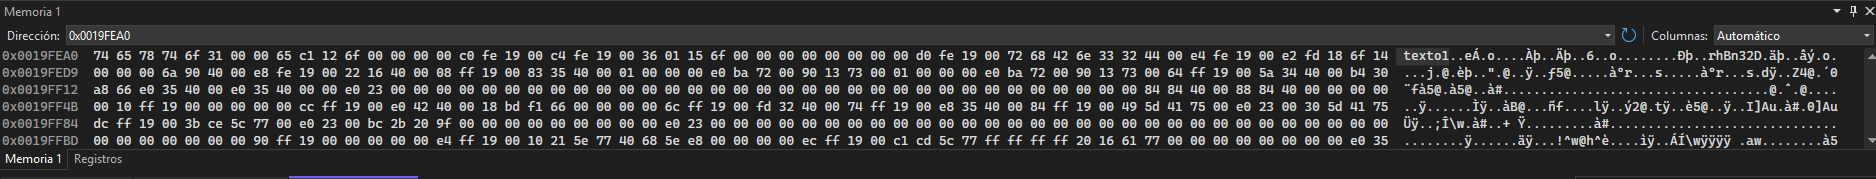
\includegraphics[width=\textwidth]{texto1Memoria.png}
  \end{center}

  Repetimos el proceso para la segunda cadena de carácteres obteniendo lo siguiente:

\begin{center}
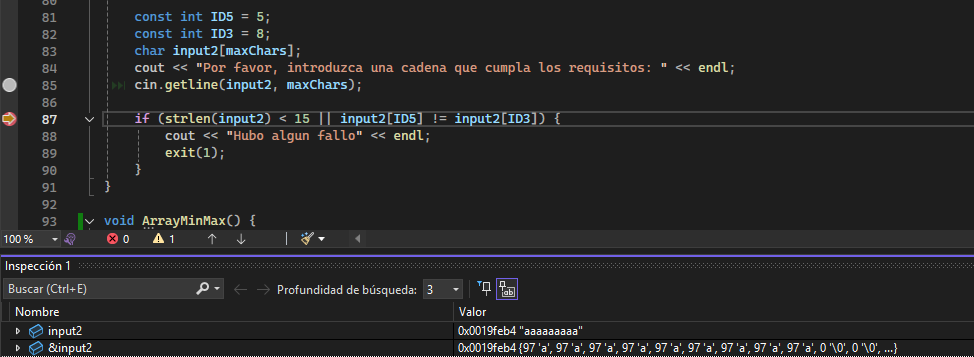
\includegraphics[width=\textwidth]{texto2.png}
\end{center}
\begin{center}
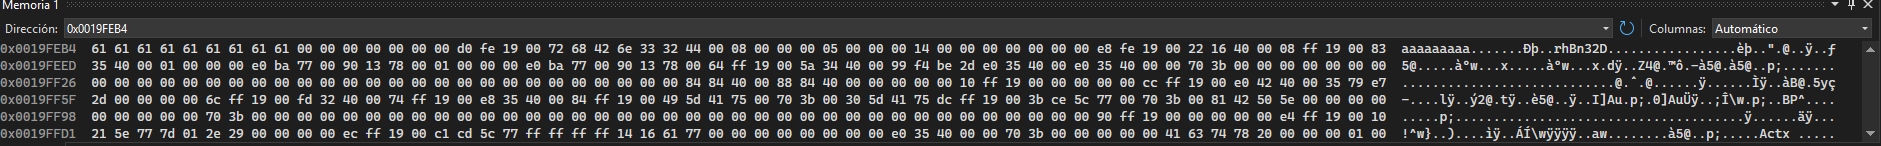
\includegraphics[width=\textwidth]{texto2Memoria.png}
\end{center}

\newpage

\subsection{Marco de pila ArrayMinMax}
Para saber el marco de pila de la función ArrayMinMax, debemos poner un punto de interrupción después de 
leer los elementos del vector. A continuación, ejecutamos el programa en modo depuración y seleccionamos la 
opción \textbf{Ventanas \(\rightarrow\) Depurar \(\rightarrow\) Memoria} y \textbf{Ventanas \(\rightarrow\) Depurar \(\rightarrow\) Registro}. 
En la ventana de memoria, introducimos la dirección de memoria de la variable que contiene el vector y en la ventana de registro, vemos en que dirección 
de memoria se encuentra el puntero de pila.
\begin{center}
  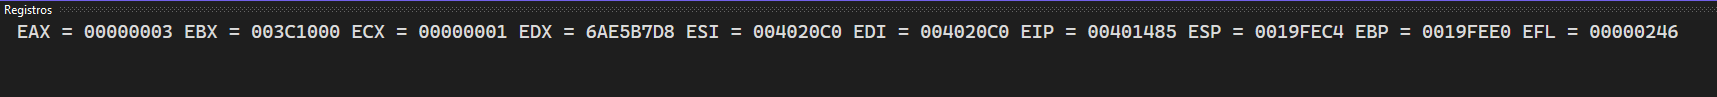
\includegraphics[width=\textwidth]{VentanaRegistros.png}
  \end{center}

\indent En nuestro caso, tenemos que la dirección de memoria de la variable que contiene el vector es \(\mathbf{0x0019FED8}\), la dirección de memoria del puntero de pila es \(\mathbf{0x0019FEE0}\) y la dirección de retorno es \(\mathbf{0x0019FEE4}\). Como se muestra en la siguiente imagen:
\begin{center}
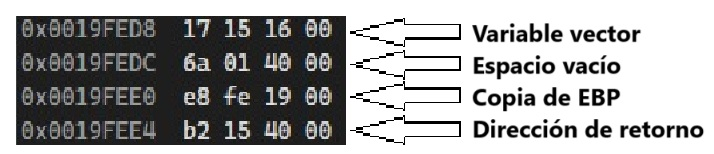
\includegraphics[width=\textwidth]{VentanaMemoria.jpg}
\end{center}

\indent Notar que hay un epsacio vacío para futuras variables locales que se van a usar en el método.


\subsection{Acceso de lectura ArrayMinMax}
Para explicar el acceso de lectura a un elemento del vector, debemos poner un punto de interrupción en la lectura 
de un elemento del vector, en nuestro caso cuando se lee el elemento cero del vector para inicializar al máximo.
 A continuación, ejecutamos el programa en modo depuración y, haciendo click derecho sobre el código, vamos al desensamblado. Como se 
 muestra en la siguiente imagen:
 \vspace{1ex}
 \begin{center}
  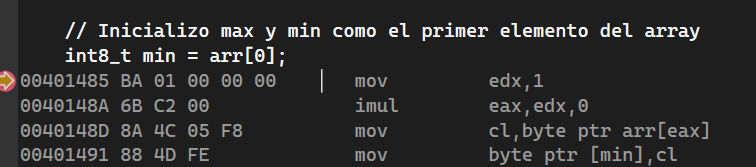
\includegraphics[width=\textwidth]{VentanaDesensamblado.png}
 \end{center}
 \vspace{1ex}
 Explicación de la imagen:
 \begin{enumerate}
  \item En la primera línea, asigna el valor 1 al registro edx.
  \item En la segunda línea, multiplica el valor del registro edx (en nuestro caso el 1) por el valor 0 (ya que estamos accediendo al primer elemento del vector) y asigna el 
  resultado al registro eax.
  \vspace{3ex}

  \item Mueve la información almacenada en la posición eax del vector (en nuestro caso es la posición 0) a la 8 bits más bajos del registro c. Omitimos la letra e de ''ecx'' para acceder a la 
  palabra más baja del registro, y ponemos ''l'' en lugar de ''x'' para acceder a los 8 bits más bajos, de ahí que escribamos ''cl'' en vez de ''ecx''.
  \item Mueve la información almacenada en la parte baja del registro ecx a la variable local de un byte denominada min.
 \end{enumerate}

\newpage

\section{División del trabajo}
A la hora de organizar el trabajo en equipo, nos reunimos todos para aportar ideas y
pensar en común los cuatro métodos. Después de plantear varias ideas y ponernos de acuerdo 
en cómo hacer cada método, nos dividimos la creación de código de la siguiente manera, siempre 
siguiendo el guion que habíamos acordado en un principio:
\begin{itemize}
  \item Andrés Fernández-Junquera Fernández: ArrayMinMax()
  \item Bruno Martín Rivera: PasswordControl()
  \item Javier Ortín Rodenas: AsmBasedControl()
  \item Mateo Rama García: CountActiveBits()
\end{itemize}

\indent Cada alumno programó su respectiva función de manera independiente y realizó una serie de pruebas para comprobar
el correcto funcionamiento del código. 
\vspace{2ex}

A continuación, trabajamos en conjunto para responder a las cuestiones, explicar el código, y redactar la memoria. También, 
se han contabilizado las horas de trabajo de cada uno de los integrantes del grupo, siendo estas las siguientes:
\begin{itemize}
  \item Andrés Fernández-Junquera Fernández: 4 horas
  \item Bruno Martín Rivera: 4 horas
  \item Javier Ortín Rodenas: 5 horas y media
  \item Mateo Rama García: 5 horas y media
\end{itemize}

\end{document}
